\documentclass{article}
\usepackage[margin=1.0in]{geometry}
\usepackage{graphicx}
\PassOptionsToPackage{hyphens}{url}\usepackage{hyperref}

\title{CS 4641: Machine Learning\\
Final Project Analysis}
\date{}
\author{}

\begin{document}
\maketitle
\section*{Introduction}
This dataset consists of EEG recordings of brain activity of 500 individuals measured over 23 periods of 1 second. This created a total of 11500 data points, and each of them were labeled from 1-5 based on whether seizure activity was recorded, whether the EEG was recorded from an area with a tumor, and  whether the patients eyes were open or not. Most previous studies focused only on the binary classification of recording seizure activity versus no seizure activity (the rest). I wanted to expand on this work by trying to use 3 class labels: presence of seizure activity, recording the area of a tumor, and neither. It would be significant for a machine learning model to be able to decide whether there is seizure activity or if it was able to detect the presence of a tumor in the recording area. This could help doctors diagnose issues more easily and non-invasively. The dataset had one point missing a class label, so this one point was removed and not used in training or evaluating models. I  evaluated the models on their performance in correctly predicting the label of unseen data, and split the data set into 80\% training and 20\% withheld test data for the hyperparameter tuning. While tuning hyperparameters for each algorithm, I withheld the same test set of data from each algorithm and evaluated the ``best" tuned model for each algorithm with this test set. 
\bigskip \\Then to do a more standardized and statistically significant comparison of performance between the tuned models, I used the full test set and used 5-fold cross validation to get a more statistically proven confidence interval for the true performance of each tuned model, and compare these score intervals between each algorithm/tuned model.
\section*{Algorithm Description}
I first tried using the Random Forest algorithm with bagging, using the RandomForestClassifier from \texttt{sci-kit learn}. Random Forests is essentially creating many decision trees randomly and the class label ``decision'' is the label that resulted from the most decision trees, sort of like a vote. In my broader search of hyperparameter values, I focused on the hyperparameters that affect the ``size and shape" of the forest: The number of estimators (the number of decision trees), the max depth of the trees, the min samples required to split an internal node, the min samples required to be in a leaf node, and the maximum samples to use in building each tree. Because I am using bagging, I have set the `bootstrap' parameter to \texttt{true} and I included the max samples in my hyperparameters. Thus, each tree in the forest will be generated by a bootstrapped sample of \texttt{max\_samples} data points.
\bigskip \\Then I tried using a Support Vector Machine, using the \texttt{SVC} class from  \texttt{sci-kit learn}. A linear support vector machine essentially tries to calculate the line that would best separate data points with different class labels while leaving the biggest margin from the line to any training data points. For my models, I did not always use a linear SVM since my data was likely not linearly separable, and applying other kernels gave me better results. This was one of the hyperparameters I looked at. Others were `C', the regularization parameter that helps to smooth the model and prevent overfitting, and `gamma', the kernel coefficient, which would affect the shape of the kernelized data.
\bigskip \\Finally, I tested the performance of neural networks using the Multi-layer Perceptron classifier from \texttt{sci-kit learn}. As described in the name, the neural network is a web of nodes or ``perceptrons" that act like neurons in the brain, triggered by an activation function to send a signal forward in the network, or not. In my first, broader search of hyperparameter values, I tested different activation functions and solver methods, as well as the L2 penalty (alpha) and most importantly, I tested a lot of variations for the structure of the hidden layers. 
\section*{Hyperparameter Tuning}
\subsection{Random Forests with Bagging}
I first ran a basic model with the default parameters set by \texttt{sci-kit learn}, to get a baseline idea of the algorithm's performance. This model took 0.27 minutes to train and score and produced a score of 0.8243 on the test data.
\bigskip \\To ``scan" a wider space of hyperparameter values within a reasonable runtime, I decided to tune my hyperparameters by first using a Random Search across the broader grid of parameter values, limited at 50 iterations and cross-validated with 3 folds. Then I picked just 2 parameters to search more thoroughly with Grid Search, paired with the other tuned hyperparameters from the random search results. So, I then ran a Random Search, which took 92.3 minutes to run and the best estimator found by the search had a cross-validation score (on the provided training data) of 0.7984, but it produced a score of 0.8190 on the reserved test data set. This best estimator had the hyperparameters: 
\begin{center}
 `max depth': 163, 
 \\`min samples leaf': 1, 
 \\`min samples split': 21, 
 \\`max features': None, 
 \\`max samples': None, 
 \\`num estimators': 726. 
 \end{center}
Here are the average scores for the 3-fold cross validation and some information about the parameters used for the top 5 performing sets of parameters: 
\begin{center}
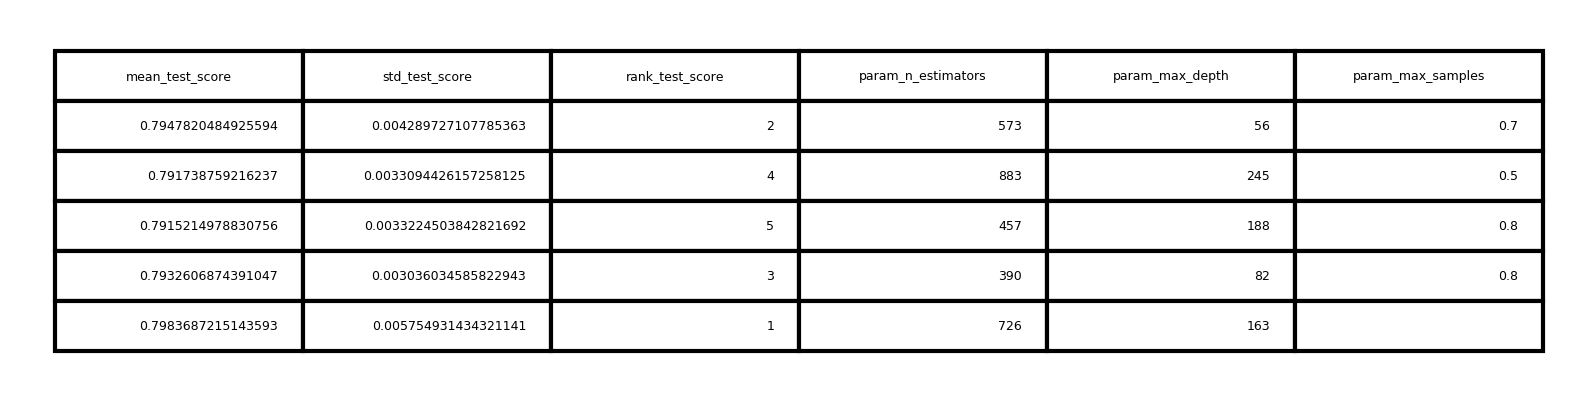
\includegraphics[scale=1.2]{RandomForestRandomSearchTable.png}
\end{center}
I noticed that the model with the tuned hyperparameters from the Random Search performed worse on the withheld test data than our default paramater model, so in my grid search I decided to search parameter values around the default values rather than the results of my random search. Those default parameters were:
\begin{center}
 `max depth': None, 
 \\`min samples leaf': 1, 
 \\`min samples split': 2, 
 \\`max features': `sqrt', 
 \\`max samples': None, 
 \\`num estimators': 100. 
 \end{center}
\bigskip For the grid search, I tuned the `num estimators' hyperparameter, which controls how many decision trees are made for the forest, and the `max features' hyperparameter, which controls the number of features considered when looking for the best split at a node in a tree. The best values for these parameters found by the grid search are $num\_estimators=110$ and $max\_features=None$.
So the overall set of best hyperparameters found from these experiments is:
\begin{center}
	 `max depth': None, 
	 \\`min samples leaf': 1, 
 	\\`min samples split': 2, 
	 \\`max features': `sqrt', 
 	\\`max samples': None, 
	 \\`num estimators': 110. 
 \end{center}
 This best estimator had a score of 0.8230 on the test data and took 65.7 minutes to run. The models tested in the search are shown in the following graph:
 \begin{center}
 	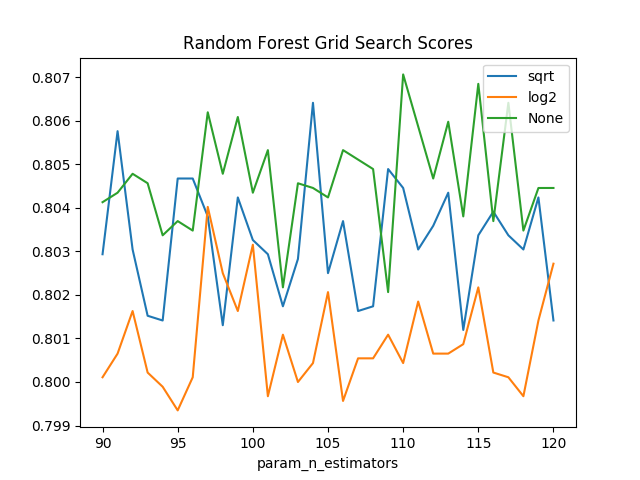
\includegraphics[scale=.7]{RandomForestGridSearch.png}
 \end{center}
There was not a clear trend in performance for the `num estimators' parameter, but generally, $max\_features=None$ performed better than `sqrt' and `log2'. This could be because the algorithm is considering more features before deciding on a best split at each node, so it is using more available information to make a more educated decision. However, this does slow down the runtime since it has to consider more features. The score on the test data for this tuned model was actually slightly lower than our first default parameter model, but testing on one set of test data does not necessarily provide the single true evaluation of a model. Later, I will test a model with this tuned set of hyperparameters with cross validation to get a more general evaluation of the performance of a model with these hyperparameters.
\subsection{Support Vector Machines}
Like with random forests, I first ran a basic model with the default parameters set by \texttt{sci-kit learn}, to get a sort of baseline evaluation. The default kernel was \texttt{rbf} and produced a score of 0.8052 on the test data and took 0.3121 minutes to fit the model.
\\I also trained a model with a linear kernel, still with all same other default parameters, to see if my data was linearly separable. The algorithm did not converge with the linear kernel, so I set the max iterations to 100,000. This model produced a score of 0.5565 on the test data, lower than the basic non-linear model, and a relatively low score overall. This indicated to me that this data set was probably not linearly separable, and it would be better to try a different kernel. This model took 39.8132 minutes to fit and score.
\\Then, like with random forests, I ran a random search with cross validation over a broad range of hyperparameters, to get an idea of a more specific area to search before using grid search on just 2 hyperparameters. The random search took 38.0 minutes to run and the best estimator found by the search had a cross-validation score (on the provided training data) of 0.8074, but it produced a score of 0.8304 on the reserved test data set. This best estimator had the hyperparameters: 
\begin{center}
`C': 22, 
\\`gamma': 'scale', 
\\`kernel': `rbf'
\end{center}
I had also searched the parameter `degree' but it is only used for the polynomial kernel so it wasn't used in this best estimator.
\\Here are the average scores for the 3-fold cross-validation and some information about the parameters used for the top 5 (with ties) performing sets of parameters: 
\begin{center}
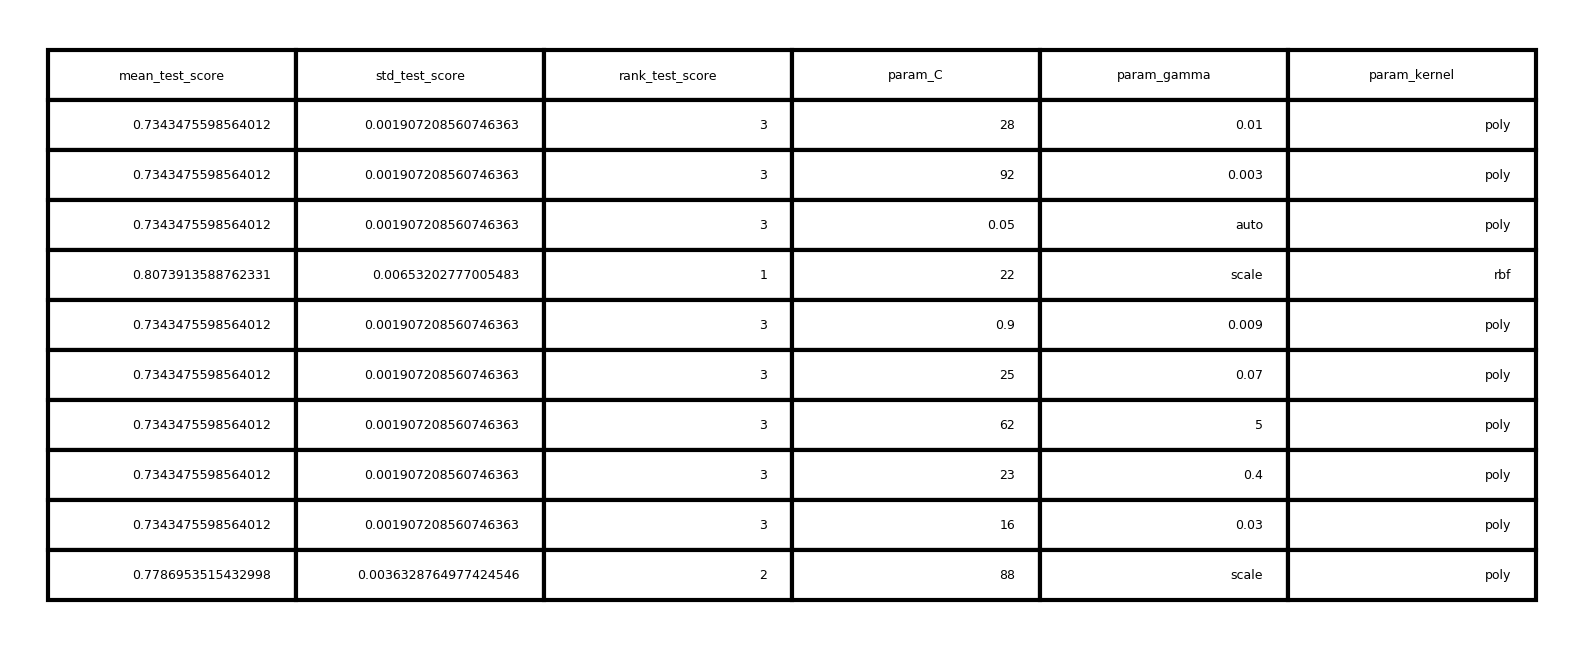
\includegraphics[scale=1.2]{SVMRandomSearchTable.png}
\end{center}
For the grid search, I tuned the regularization hyperparameter `C', and `gamma' the kernel coefficient hyperparameter. The best values for these parameters found by the grid search are $C=31$ and $gamma=scale$.
So the overall set of best hyperparameters found from these experiments is:
\begin{center}
`C': 31, 
\\`gamma': 'scale', 
\\`kernel': `rbf'
\end{center}
 This best estimator had a score of 0.8326 on the test data and took 29.0 minutes to run. The models tested in the search are shown in the following graph:
 \begin{center}
 	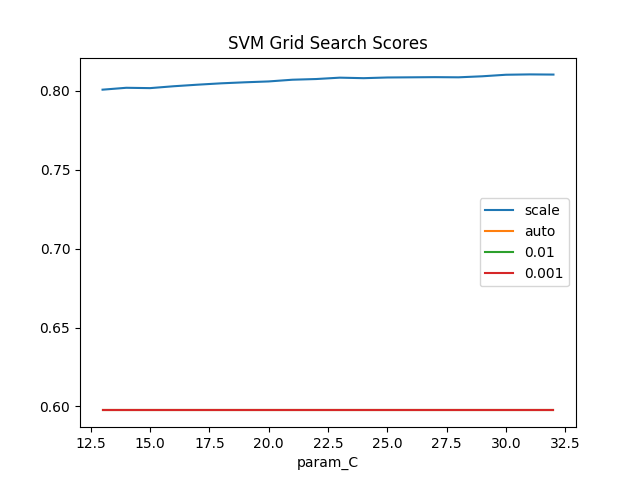
\includegraphics[scale=.7]{SVMGridSearch.png}
 \end{center}
 The lines for the gamma values 0.01 and \texttt{auto} are the same flat line as for gamma value 0.001, so it is hidden by that line. It is clear that the gamma value \texttt{scale} performed much better than the other gamma values, though there isn't much change as C increases, though it increases slightly.
The score on the test data for this tuned model was better than for any SVM model in our previous experiments.
\subsection{Neural Networks}
Again, I first ran a basic model with the default parameters for neural networks. However, the default used only one hidden layer of 100 nodes, so I expanded this to two hidden layers of 100 nodes. This model produced a score of 0.7078 on the test data set and took 0.2487 minutes to fit the model and score on the test data.
\bigskip \\Then, like with the previous two algorithms, I ran a random search with cross validation over a broad range of hyperparameters, to get an idea of a more specific area to search using grid search on just 2 parameters. The random search took 97.7 minutes to run and the best estimator found by the search had a cross-validation score (on the provided training data) of 0.7746, but it produced a score of 0.7865 on the test data set. This best estimator had the hyperparameters:
\begin{center}
`activation': `relu',
\\`alpha': 0.006,
\\`hidden layer sizes': (230, 310, 430, 140),
\\`learning rate init': 0.006,
\\`solver': `adam'. 
\end{center}
While values for the parameter learning rate was also searched, it is not used with the solver \texttt{adam} so the value returned for this parameters does not actually affect the model.
\\Here are the average scores for the 3-fold cross validation and some information about the parameters used for the top 5 performing sets of parameters: 
\\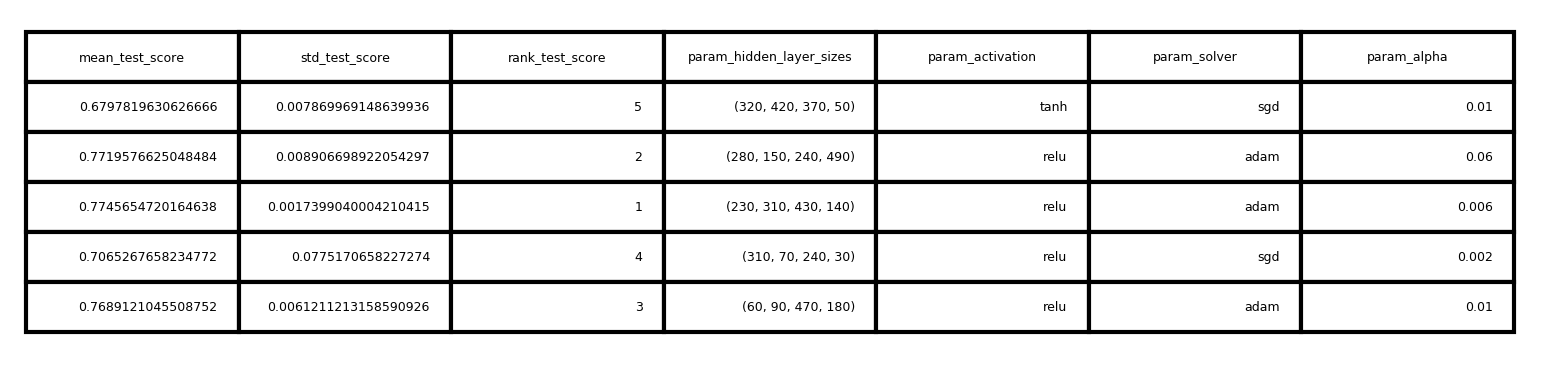
\includegraphics[scale=1.3]{NeuralNetRandomSearchTable.png}
For the grid search, I tuned the number of perceptrons in each of 4 hidden layers (since the random search returned a model with 4 hidden layers) and `alpha', the L2 penalty. The best values found for these parameters found by the grid search are `alpha': 0.007,and `hidden layer sizes': (230, 313, 430, 143). So the overall tuned hyperparameters for the neural network are: 
\begin{center}
`activation': `relu',
\\`alpha': 0.007,
\\`hidden layer sizes': (230, 313, 430, 143),
\\`learning rate init': 0.006,
\\`solver': `adam'. 
\end{center}
This best estimator had a score of 0.8056 on the test data and the grid search took 400.3 minutes to run. The top 5 peroforming models tested in the search are shown in the following table:
\begin{center}
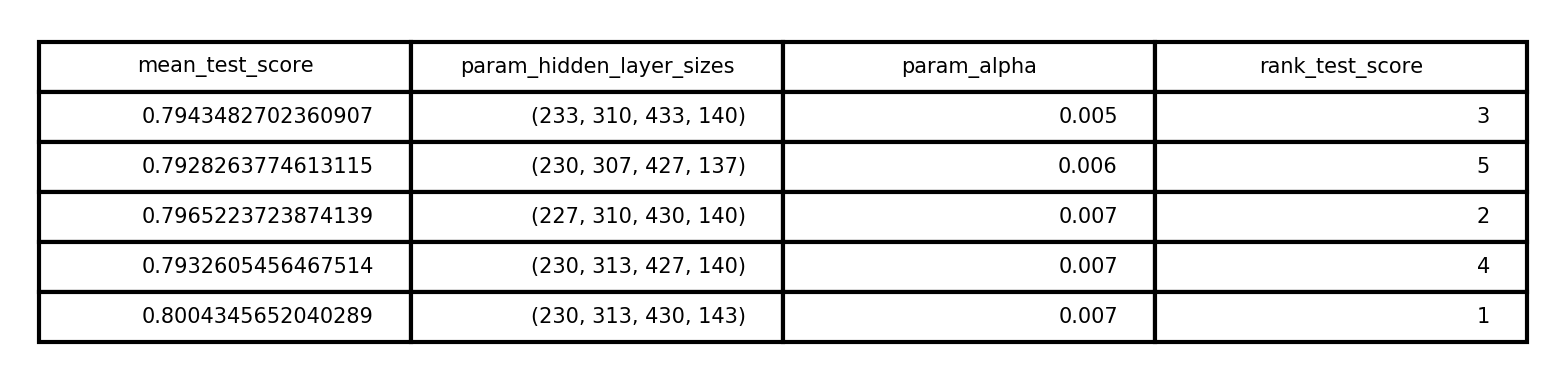
\includegraphics[scale=1.3]{NeuralNetGridSearchTable.png}
\end{center}
and all sets of hyperparameters searched can be visualized in the following graph:
\begin{center}
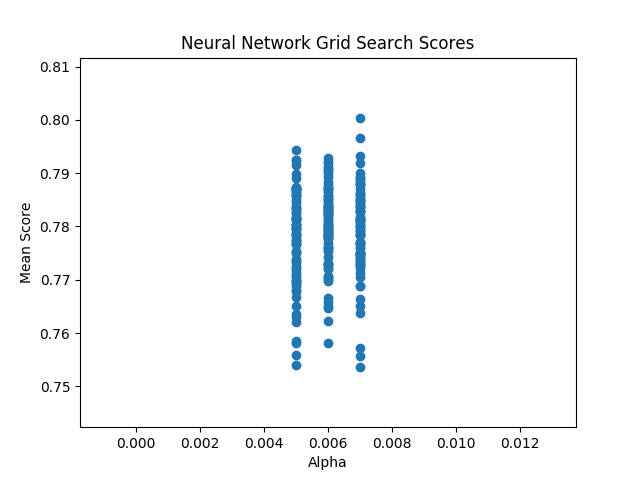
\includegraphics[scale=.7]{NNGridSearch.png}
\end{center}
where each point is a model with one set of hyperparameters from the grid search space. While we can't see the hidden layer sizes used for each model, we can see that each value of alpha produced models with generally the same range of performance, but the highest alpha tested, 0.007, had a slightly more varied performance in models and a few happened to outperform the rest. It could be that higher L2 regularization (alpha) helped prevent overfitting, and was most effective at regularization with that particular neural network ``layer shape".
\section*{Performance Comparison}
I tried to use a simple method to evaluate the performance of the best estimators on an even playing field during hyperparameter tuning by scoring all models on the same withheld test set. To get a more statistically significant understanding of the performance of my tuned models for each of these algorithms, however, I decided to run 5-fold Cross Validation on each of the algorithms using the tuned hyperparameters.
\bigskip \\For the Random Forest algorithm, this resulted in a mean score of 0.8119 with a standard deviation of 0.00348. Because I only have 5 samples, I used the \texttt{t} distribution to find a confidence interval. I calculated that I can be 95\% confident that the true score of this model (that is, its performance if it was used to predict on every data point in the input space) is between 0.8086 and 0.8152.
\\bigskip \\For the Support Vector Machine algorithm, cross validation resulted in a mean score of 0.8116 with a standard deviation of 0.00369. Using the same method as for Random Forests, I calculated that I can be 95\% confident that the true score of this model is between 0.8081 and 0.8151. 
\bigskip \\For the Neural Network algorithm, cross validation resulted in a mean score of 0.8004 with a standard deviation of 0.00618. Using the same method as the previous two algorithms, I calculated that I can be 95\% confident that the true score of this model is between 0.7945 and .8063.
\bigskip \\Overall, the performance of the three tuned models weren't drastically different, though the Neural Network was slightly worse. Between support vector machines and random forests, both algorithms performed nearly equally as well, but random forests has a slightly narrower confidence interval with some higher values than support vector machine. Thus I would argue that the best algorithm for this problem is Random Forests.
\section*{Conclusion}
As I explained in the previous section, the best performing algorithm (by a narrow margin) would be Random Forests. It also had the shortest fit and score time, when compared to SVMs and Neural Networks. Neural Networks were by far the slowest to fit and score, making it somewhat impractical for real world use, and it didn't perform as well as Random Forests anyway. Random Forests and Neural Networks both had lots of hyperparameters that influenced the shape of the graphs generated by the algorithm, things like the number of trees in the forest or depth of each tree, and the hidden layer sizes and number of hidden layers for neural nets). In that way, the hyperparameters were simpler and shorter for SVM, since we mostly focused on tuning the level of regularization or the shape of the kernel function. Overall though, Random Forests are quick and performed well with this dataset, and would be the best to use in the real world for this domain.
\section*{Acknowlegements}
I used the following sites to help me write code for this project:
\begin{itemize}
\item \url{https://towardsdatascience.com/hyperparameter-tuning-the-random-forest-in-python-using-scikit-learn-28d2aa77dd74} for understanding hyperparameter tuning with Sci-Kit Learn.
\item \url{http://jonathansoma.com/lede/algorithms-2017/classes/fuzziness-matplotlib/understand-df-plot-in-pandas/} for pandas and plotting
\item \url{https://scikit-learn.org/stable/modules/cross_validation.html} for understanding cross validation and evaluating model performance.
\end{itemize}
As well as the documentation for \texttt{sci-kit learn}, \texttt{pandas} and \texttt{matplotlib}.
\end{document}